\documentclass[a4paper,11pt]{article}

\usepackage[T1]{fontenc}
\usepackage[utf8]{inputenc}
\usepackage{lmodern}
\usepackage[margin=1in]{geometry}
\usepackage{amsmath,amssymb}
\usepackage{graphicx}
\usepackage{booktabs}
\usepackage{siunitx}
\usepackage{tabularx}
\usepackage{float}
\usepackage[protrusion=true,expansion=false]{microtype}
\usepackage[hidelinks]{hyperref}

\sisetup{separate-uncertainty=true}
\graphicspath{{figures/}}
\newcommand{\familyone}{Classical Hall-Petch}
\newcommand{\familytwo}{Physics-derived descriptors}
\newcommand{\familythree}{Composition/processing}
\newcommand{\familyfour}{Non-linear ML (ARMOTE-CV)}
\newcommand{\familyfive}{Symbolic regression}
\renewcommand{\thesection}{S\arabic{section}}
\renewcommand{\thetable}{S\arabic{table}}
\renewcommand{\thefigure}{S\arabic{figure}}
\renewcommand{\theequation}{S\arabic{equation}}
\setlength{\emergencystretch}{3em}

\title{Supplementary Information for:\\
\emph{Revisiting Hall--Petch strengthening in FCC multi-principal-element alloys: Best practices for building and auditing machine-learning strength models}}
\author{Mrinalini~Mulukutla$^{1,*}$, Shakti~Prasad~Padhy$^{2}$, Douglas~Allaire$^{2}$,\\
Ibrahim~Karaman$^{1}$, Raymundo~Arr\'{o}yave$^{1,2}$\\[0.5em]
\small $^{1}$Department of Materials Science and Engineering, Texas A\&M University,\\
\small College Station, TX 77843, USA\\
\small $^{2}$J. Mike Walker '66 Department of Mechanical Engineering, Texas A\&M University,\\
\small College Station, TX 77843, USA\\
\small $^{*}$Corresponding author: mrinalini.mulukutla@tamu.edu}
\date{}

\begin{document}
\maketitle
\begingroup
\sloppy
\tableofcontents
\endgroup

This Supplementary Information follows the same fixed model-family hierarchy as Fig.~1 of the main paper: Family~1 (\familyone), Family~2 (\familytwo), Family~3 (\familythree), Family~4 (\familyfour), and Family~5 (\familyfive). The names and order remain unchanged in both documents. S1--S4 are cumulative input sets within Family~4, not separate model families. E1--E3 are literature evidence classes and are also separate from the model hierarchy.

Primary internal performance is reported using shuffled 5-fold cross-validation, leave-one-out (LOO), and leave-one-batch-out (LOBO) validation. LOO operates at the record level. When a composition is repeated, another record with the same composition can remain in the training set. We therefore do not describe LOO as strict unseen-composition validation. LOBO tests transfer to a new Bayesian-optimization iteration. External literature testing and singularity audits of closed-form equations are reported separately from internal predictive validation.

\section{Dataset audit and exploratory analysis}
\label{si:data}

\subsection{Campaign provenance, synthesis, and characterization}

The broader alloy-discovery effort began with Campaign A, which established the closed-loop, multi-objective workflow~\cite{Hastings2025FCC}. Campaign A is a methodological prequel and does not contribute records to the present property-modeling dataset. This dataset combines the subsequent B and C Bayesian-optimization campaigns carried out at Texas A\&M University through the BIRDSHOT initiative within the ARL HTMDEC program~\cite{Mulukutla2024BIRDSHOT,Mulukutla2026BRAVE}. The B campaign contributes 35 records from batches BBA, BBB, and BBC, including 34 with YS. It explored the Al--Co--Cr--Cu--Fe--Mn--Ni--V system under an FCC phase-stability constraint while holding processing fixed. Section~2.2 of Ref.~\cite{Mulukutla2026BRAVE} documents the B-campaign synthesis and specimen-preparation workflow.

The C campaign contributes 59 records from CBA, CBB, and CBC. It used insights from the B campaign to focus on V--Cr--Mn--Fe--Co--Ni alloys and jointly varied composition, cold work, recrystallization temperature, and hold time. During design-space curation, a modified JMAK-type static-recrystallization and grain-growth prior provided grain-size estimates for feasible candidates. The complete C-campaign and grain-growth-model details will be reported separately. The present regression analysis uses measured EBSD grain sizes rather than the design-stage estimates.

Both campaigns followed the same high-level route of vacuum-arc melting from high-purity elements, homogenization, cold rolling, recrystallization, and quenching. EDS and XRD checked realized chemistry and phase constitution; SEM and EBSD documented the microstructure; and quasistatic tensile and Vickers indentation measurements supplied YS and HV. Figure~2 of the main paper shows representative chemistry and microstructure verification. Figure~\ref{fig:provenance} shows the non-uniform composition and processing coverage that motivates grouped validation.

\begin{figure}[H]
  \centering
  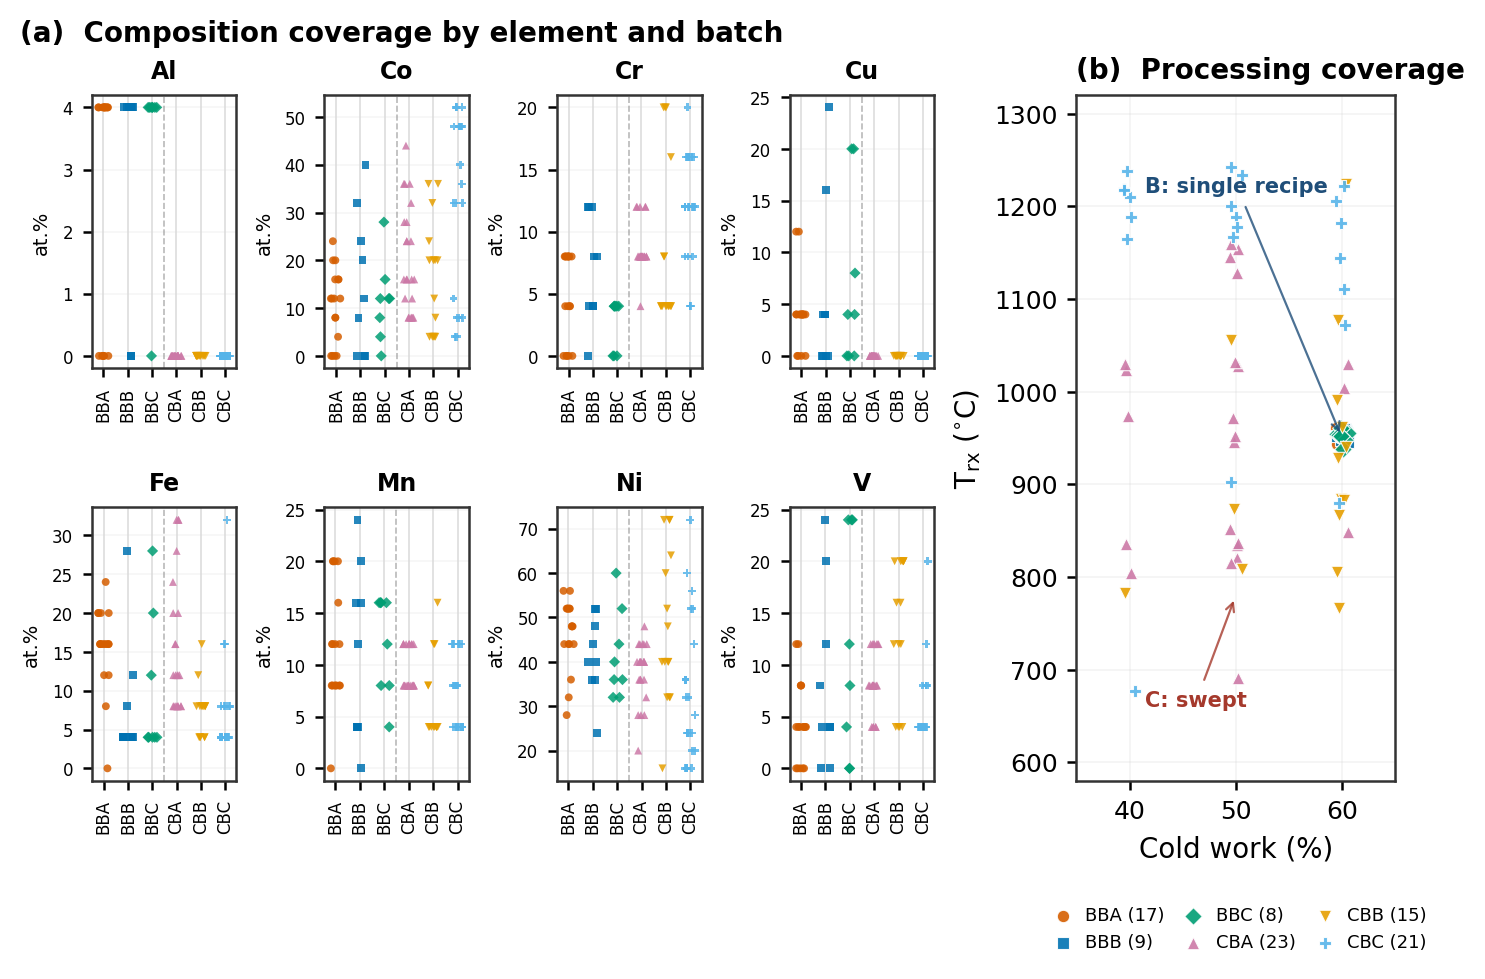
\includegraphics[width=0.96\textwidth]{fig_provenance.png}
  \caption{Composition and processing coverage by batch. The B campaign uses one fixed processing condition, while the C campaign spans a processing grid. The coverage follows the experimental design and is not a random sample of the composition simplex.}
  \label{fig:provenance}
\end{figure}

\subsection{Audited record structure and distributions}

The source workbook contains 94 records and 19 original columns. Every composition row sums to 100~at.\% (Table~\ref{tab:data}). YS is available for 93 records, and HV is available for all 94. BBA09 is the only record without YS. The B batches contain 35 hardness records and 34 YS records. The C batches contain 59 records for both targets. Processing is fixed within the B campaign, whereas the C campaign varies cold work, recrystallization temperature, and hold time together with composition.

\begin{table}[H]
\centering
\caption{Audited dataset statistics. Means and standard deviations are sample statistics.}
\label{tab:data}
\begin{tabular}{lrrrr}
\toprule
Quantity & $n$ & Min & Max & Mean $\pm$ SD \\
\midrule
YS (MPa) & 93 & 151.5 & 544.5 & $268.5\pm81.6$ \\
HV & 94 & 57.6 & 227.5 & $133.9\pm33.6$ \\
$d$ ($\mu$m) & 94 & 14.66 & 211.75 & $57.39\pm42.67$ \\
$\mathrm{SD}_{\mathrm{grain}}$ ($\mu$m) & 94 & 8.32 & 321.06 & $44.72\pm44.83$ \\
\bottomrule
\end{tabular}
\end{table}

The full dataset contains 82 unique compositions. The 93-record YS subset contains 81. Nine composition groups are repeated and account for 21 records. One composition, Co$_4$Cr$_4$Fe$_4$Mn$_4$Ni$_{72}$V$_{12}$, appears in both CBB and CBC, with three CBB records and one CBC record. Record-level LOO can therefore contain exact-composition overlap. LOBO reduces this overlap but does not remove it completely. We report these facts as part of the validation audit rather than treating them as another validation protocol.

Mean grain size and its standard deviation are strongly correlated ($r=0.801$). The dimensionless coefficient of variation, $\mathrm{SD}_{\mathrm{grain}}/d$, ranges from 0.47 to 2.99. A claim that distribution width has an independent physical role should therefore compare raw SD with normalized width and with distribution moments such as $E[d^{-1/2}]$.

The source data also contain measurement scatter, which is distinct from grain-distribution width. $\mathrm{SD}_{YS}$ is available for 80 records and ranges from 0.2 to \SI{98.7}{MPa}; $\mathrm{SD}_{HV}$ is available for all 94 and ranges from 1.43 to 12.44 HV. These values are not used as model features because replicate counts and reporting definitions are not consistent across records. In contrast, $\mathrm{SD}_{\mathrm{grain}}$ is an EBSD microstructure descriptor and is evaluated explicitly as a predictor.

The strongest composition--grain-size correlations include $r(d,c_{\mathrm{Cr}})=+0.38$ and $r(d,c_{\mathrm{Al}})=-0.32$. On average, Cr-rich alloys are therefore coarser and Al-rich alloys are finer. These signs were reversed in the earlier draft. A regression of $d^{-1/2}$ on composition explains approximately 40\% of its variance. Adding processing raises this value to approximately 54\%. Composition and grain size are therefore not experimentally orthogonal.

Figure~\ref{fig:distributions} shows the global property distributions. The gap in the grain-size histogram comes from the C-campaign processing grid and the B campaign's fixed recipe. It is not evidence of a bimodal grain-growth mechanism. Figure~\ref{fig:tensile} shows the C-campaign true stress--strain curves used to extract 0.2\% offset YS. Figure~\ref{fig:correlation} summarizes correlations among composition, processing, and descriptors. Several deterministic descriptors are strongly correlated with one another, so coefficient and feature-importance interpretations must account for redundancy.

\begin{figure}[H]
  \centering
  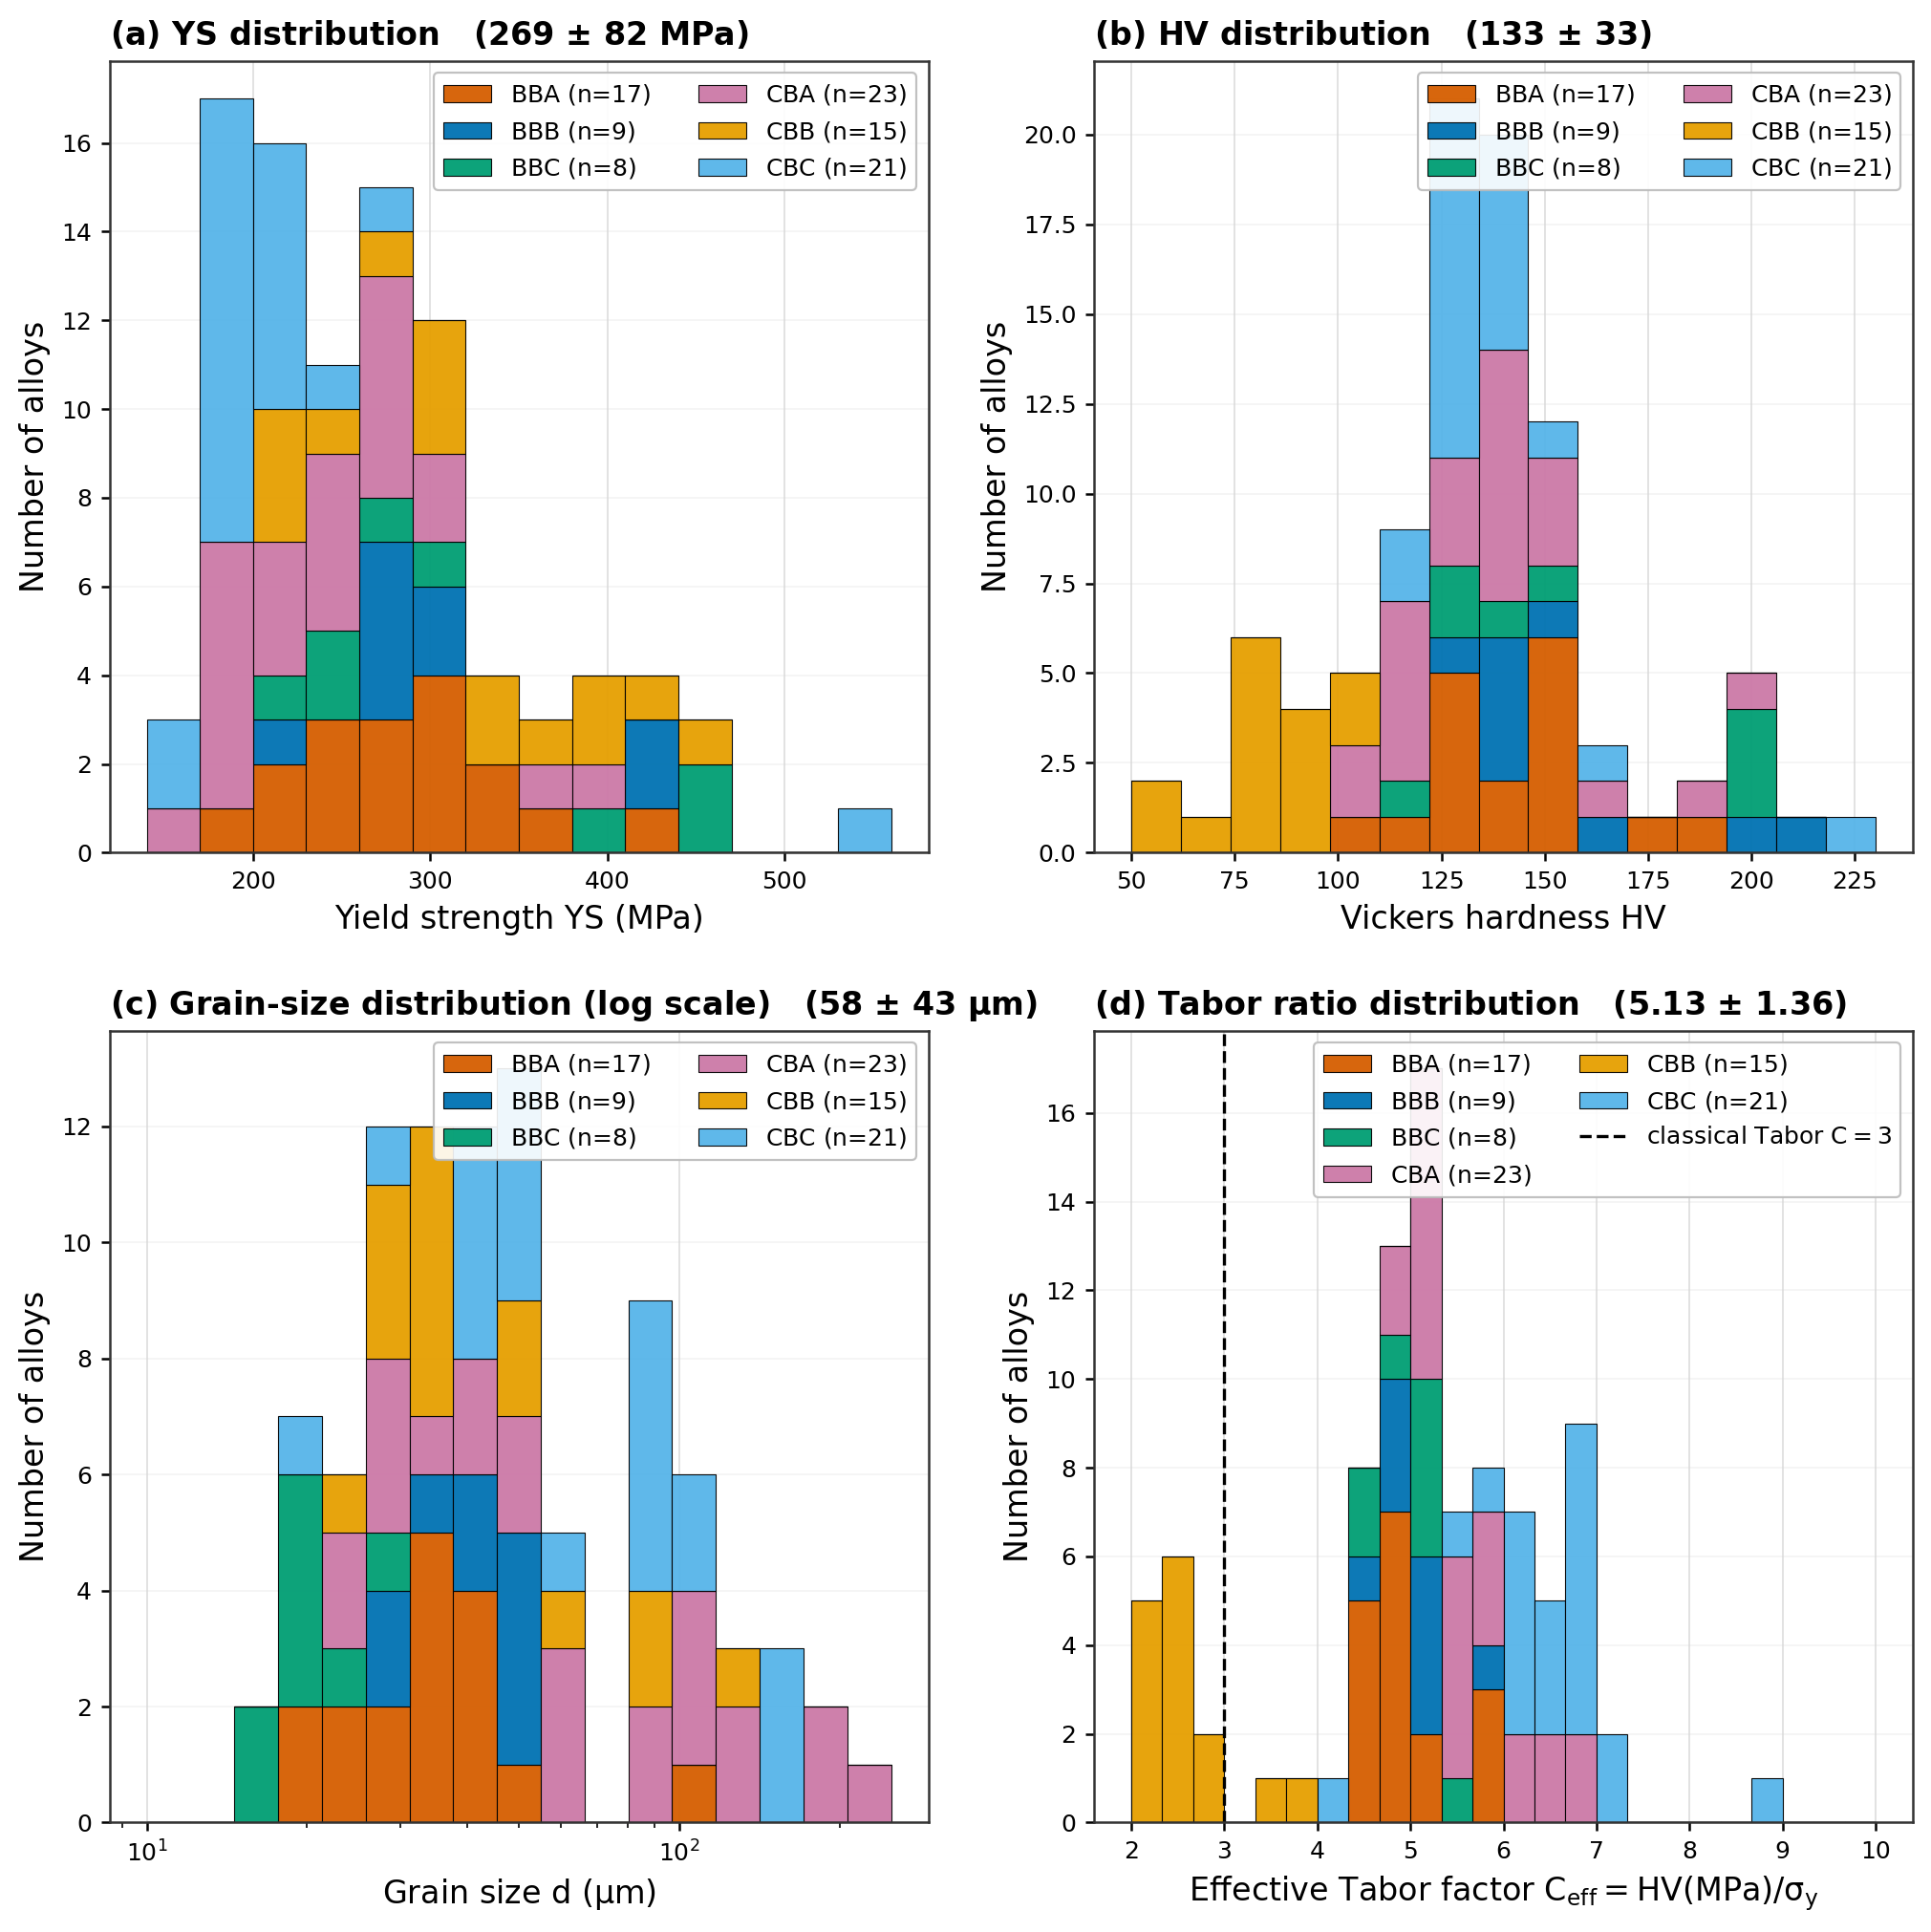
\includegraphics[width=0.72\textwidth]{fig_property_histograms.png}
  \caption{Audited YS, HV, grain-size, and effective hardness-to-yield distributions by batch.}
  \label{fig:distributions}
\end{figure}

\begin{figure}[H]
  \centering
  \includegraphics[width=0.72\textwidth]{tensile_tests.png}
  \caption{True stress--strain curves for the C-campaign records at a nominal strain rate of $5\times10^{-4}$~s$^{-1}$. The 0.2\% offset values are the YS targets used in the analysis.}
  \label{fig:tensile}
\end{figure}

\begin{figure}[H]
  \centering
  
\includegraphics[width=0.80\textwidth]{fig02_correlation_matrix.png}
  \caption{Pearson correlation matrix for composition, processing, grain-size, and descriptor variables. Correlation is descriptive and does not establish independent mechanistic effects.}
  \label{fig:correlation}
\end{figure}

\subsection{Grouped-validation conventions and primary results}
\label{si:validation}

For every protocol, predictions from all held-out records are pooled before calculating
\begin{equation}
Q^2=1-\frac{\sum_i(y_i-\hat y_i)^2}{\sum_i(y_i-\bar y)^2}.
\end{equation}
The manuscript reports this pooled quantity as cross-validated $R^2$. It is not the mean of the fold-specific $R^2$ values; Table~\ref{tab:grouped} lists the pooled scores for every model. Preprocessing is fit within each training fold. To calculate batch-clustered intervals, the six batches are resampled with replacement 1000 times while each batch remains intact. Because there are only six clusters, these intervals show sensitivity to the sampled batches but are not precise inferential confidence intervals.

\begin{table}[H]
\centering
\caption{Primary grouped-validation results reproduced by the revision-specific validation script. The Family~5 HV result is conditional on an equation structure selected using the complete dataset before the coefficients were refit in each fold.}
\label{tab:grouped}
\small
\setlength{\tabcolsep}{4pt}
\begin{tabular}{lllrrr}
\toprule
Target & Family/model & Status & 5-fold & LOO & LOBO \\
\midrule
YS & F1 Classical HP & baseline & 0.405 & 0.406 & 0.373 \\
YS & F2 PCA-OLS & fold-contained & 0.462 & 0.480 & 0.362 \\
YS & F3 M3 & pre-specified & 0.666 & 0.652 & 0.625 \\
YS & F3 M15 SD interaction & pre-specified & 0.731 & 0.694 & 0.694 \\
YS & F4 Lasso S2 & fixed settings & 0.683 & 0.674 & 0.621 \\
YS & F4 LightGBM S2 & fixed settings & 0.632 & 0.574 & 0.615 \\
HV & F1 Classical HP & baseline & 0.086 & 0.136 & $-0.077$ \\
HV & F4 LightGBM S1 & fixed settings & 0.195 & 0.323 & 0.112 \\
HV & F5 fixed form & post-selected & 0.725 & 0.727 & 0.636 \\
\bottomrule
\end{tabular}
\end{table}

The validation hierarchy changes the scientific interpretation. LOO measures record-level interpolation and can benefit from repeated or nearby compositions. LOBO tests a new iteration while retaining the practices shared across the broader program, and is therefore the primary internal grouped-transfer test. The literature stress test asks a different question about numerical behavior on heterogeneous published records, while singularity auditing checks whether a closed form remains finite and bounded over the audited domain.

\subsection{Why no hard predictive ceiling is reported}

The source analysis contained two incompatible ceiling calculations. If every singleton composition is assigned zero residual, an in-sample composition-mean oracle gives approximately $R^2=0.86$. If variance is pooled only from repeated compositions, the within-composition variance is approximately \SI{6979}{MPa^2}. This is slightly larger than the total YS variance of \SI{6651}{MPa^2}, giving a formal value near $-0.05$. Neither value is a defensible out-of-sample ceiling. There are 72 singleton YS compositions, and the repeated groups also differ in grain size and processing.

Similarly, $1-\langle\mathrm{SD}_{YS}^2\rangle/\mathrm{Var}(YS)\approx0.97$ is not a universal noise ceiling. This calculation assumes that the reported within-alloy standard deviations are irreducible errors in the modeled target. If the target is a replicate mean, its sampling uncertainty depends on the number of replicates through $\mathrm{SD}/\sqrt{n}$. A measurement-limited ceiling cannot be estimated without replicate-level measurements and replicate counts.

\subsection{Batch coverage in composition space}

Six principal components are needed to capture approximately 95\% of the composition variance. In the PC1--PC2 projection, the mean pairwise convex-hull overlap is approximately 0.21 (Fig.~\ref{fig:hulls}). This two-dimensional diagnostic does not prove support in the full composition space, but it explains why the LOBO folds differ in difficulty. CBC is relatively isolated, while CBA is well covered by the remaining batches. The aggregate LOBO score therefore combines near-interpolation with genuine extrapolation. It should be read together with the per-batch results in Table~\ref{tab:batch}.

\begin{figure}[H]
  \centering
  
\includegraphics[width=0.96\textwidth]{fig_premodel_hulls_heatmap.png}
  \caption{Batch coverage in the PC1--PC2 projection of composition space: batch convex hulls (left) and pairwise hull containment (right). These values depend on the projection and do not guarantee support in the full composition space.}
  \label{fig:hulls}
\end{figure}

\section{Family 1: \familyone}
\label{si:scaling}

Nine pre-specified scaling laws were fit to YS (Table~\ref{tab:scalinglaws}). Five monotonic laws fall within $\Delta\mathrm{BIC}<2$ of the classical Hall--Petch form. The optimized exponent is $n=0.548$. Its Bayesian posterior is $0.53\pm0.16$, with a 94\% HDI of approximately $[0.22,0.82]$. These results support $d^{-1/2}$ as a simple baseline but do not statistically rule out nearby exponents.

\begin{table}[H]
\centering
\caption{Family~1 comparison of pre-specified grain-size laws for YS, ranked by BIC. Here, $p$ is the number of fitted regression coefficients.}
\label{tab:scalinglaws}
\small
\begin{tabular}{lrrrrrr}
\toprule
Scaling law $f(d)$ & $p$ & Train $R^2$ & LOO $R^2$ & LOO RMSE & BIC & $\Delta$BIC \\
\midrule
$d^{-1/2}$ (Hall--Petch) & 2 & 0.429 & 0.406 & 62.5 & 774.5 & 0.0 \\
$\ln(d)/d$ & 2 & 0.429 & 0.406 & 62.5 & 774.5 & 0.0 \\
$d^{-2/3}$ & 2 & 0.429 & 0.405 & 62.6 & 774.6 & 0.1 \\
$d^{-1/3}$ & 2 & 0.427 & 0.403 & 62.6 & 774.9 & 0.4 \\
$d^{-1}$ & 2 & 0.419 & 0.395 & 63.1 & 776.1 & 1.6 \\
$\ln(d)$ & 2 & 0.413 & 0.388 & 63.4 & 777.2 & 2.7 \\
$d^{-0.548}$ & 3 & 0.430 & 0.406 & 62.5 & 779.0 & 4.5 \\
$d^{-1/2}+d^{-1}$ & 3 & 0.430 & 0.395 & 63.1 & 779.0 & 4.5 \\
$d^{-1}+d^{-2}$ & 3 & 0.429 & 0.387 & 63.5 & 779.1 & 4.6 \\
\bottomrule
\end{tabular}
\end{table}

\begin{table}[H]
\centering
\caption{Bayesian PSIS-LOO comparison for the Family~1 YS laws. The stacking solution is reported but is not treated as proof of a unique law.}
\label{tab:bayesian}
\small
\begin{tabular}{lrrrr}
\toprule
Model & elpd$_{\mathrm{loo}}$ & $\Delta$LOO & $p_{\mathrm{loo}}$ & Weight \\
\midrule
Hall--Petch $d^{-1/2}$ & $-518.5$ & 0.0 & 4.2 & 1.000 \\
Composite $d^{-1/2}+d^{-1}$ & $-518.5$ & 0.1 & 4.2 & 0.000 \\
Critical-thickness $\ln(d)/d$ & $-518.5$ & 0.1 & 4.3 & 0.000 \\
Intermediate $d^{-2/3}$ & $-518.7$ & 0.2 & 4.4 & 0.000 \\
Baldwin $d^{-1/3}$ & $-518.7$ & 0.2 & 4.2 & 0.000 \\
Optimized exponent $d^{-n}$ & $-518.8$ & 0.3 & 4.5 & 0.000 \\
Logarithmic $\ln(d)$ & $-519.7$ & 1.2 & 3.9 & 0.000 \\
Dunstan--Bushby $d^{-1}$ & $-520.3$ & 1.8 & 4.3 & 0.000 \\
\bottomrule
\end{tabular}
\end{table}

The classical YS baseline gives LOO/LOBO $R^2=0.406/0.373$ (Fig.~\ref{fig:scaling}). For HV, the corresponding values are $0.136/-0.077$. Mean grain size is therefore a useful YS baseline within the sampled program, but it does not transfer reliably across batches for HV.

\begin{figure}[H]
  \centering
  
\includegraphics[width=0.82\textwidth]{fig_scaling_deltabic.png}
  \caption{Information-criterion differences among pre-specified YS grain-size laws.}
  \label{fig:scaling}
\end{figure}

The Bayesian comparison is summarized in Table~\ref{tab:bayesian}, with the fitted laws in Fig.~\ref{fig:scalingfits}, the free-exponent posterior in Fig.~\ref{fig:exponent}, and the model weights in Fig.~\ref{fig:bma}. The Bayesian stacking weight concentrates on the classical form, even though several candidate laws have almost identical expected log predictive density. We therefore do not treat this boundary solution as decisive evidence for one exponent. Parameter counting also differs across the stored tables. Some Bayesian tables include the noise parameter, while the frequentist BIC tables count regression coefficients. The revised manuscript compares models only within internally consistent tables.

\begin{figure}[H]
  \centering
  
\includegraphics[width=0.64\textwidth]{fig_scaling_fits.png}
  \caption{Top Family~1 YS scaling laws over the observed grain-size range. Their close overlap shows why the data do not identify a unique exponent.}
  \label{fig:scalingfits}
\end{figure}

\begin{figure}[H]
  \centering
  \includegraphics[width=0.64\textwidth]{fig_bayesian_n.png}
  \caption{Posterior distribution of the free grain-size exponent $n$ in $\sigma_y=\sigma_0+kd^{-n}$; the dashed line marks $n=0.5$.}
  \label{fig:exponent}
\end{figure}

\begin{figure}[H]
  \centering
  
\includegraphics[width=0.64\textwidth]{fig_bayesian_bma.png}
  \caption{Bayesian model-averaged grain-only prediction with its 94\% credible band. The large residual scatter shows that grain size alone does not capture the dominant property variation.}
  \label{fig:bma}
\end{figure}

The within-replicate analysis (Table~\ref{tab:withingroup}) gives local slopes from approximately $-8539$ to 9282 in Hall--Petch units. The fixed-effect pooled slope is near 2144, with Cochran $Q\approx251$ and $I^2=96.8\%$. This apparent heterogeneity cannot be attributed to composition because most groups contain only two records and processing is not held fixed. In addition, the two-stage $k_{\mathrm{eff}}$ regression subtracts an intercept from a model that already assumes constant $k$. The supported conclusion is that constant-slope M3 is the best predictive model in Family~3. This design cannot identify variation in $k_{\mathrm{HP}}$.

\begin{table}[H]
\centering
\caption{Descriptive within-composition fits for the nine repeated-composition groups (21 records). The values compare transformations after group demeaning but do not identify composition-specific slopes.}
\label{tab:withingroup}
\small
\begin{tabular}{lrr}
\toprule
Scaling law & Pooled within-group $R^2$ & $R^2$ for the $n=3$ group \\
\midrule
$d^{-1/2}$ & 0.778 & 0.995 \\
$d^{-1/3}$ & 0.781 & 0.997 \\
$d^{-2/3}$ & 0.775 & 0.993 \\
$d^{-1}$ & 0.769 & 0.987 \\
$\ln(d)/d$ & 0.776 & 0.993 \\
$\ln d$ & 0.786 & 0.999 \\
\bottomrule
\end{tabular}
\end{table}

\begin{table}[H]
\centering
\caption{Family~1 grain-size laws fit separately to HV. The optimized exponent was selected using the full dataset and is descriptive.}
\label{tab:hvscaling}
\small
\begin{tabular}{lrrrr}
\toprule
Scaling law $f(d)$ & $p$ & Train $R^2$ & LOO $R^2$ & $\Delta$BIC \\
\midrule
$d^{-1.728}$ & 3 & 0.193 & 0.166 & 0.0 \\
$d^{-1}$ & 2 & 0.185 & 0.154 & 0.9 \\
$d^{-2/3}$ & 2 & 0.175 & 0.143 & 2.1 \\
$\ln(d)/d$ & 2 & 0.174 & 0.141 & 2.3 \\
$d^{-1/2}$ & 2 & 0.169 & 0.136 & 2.8 \\
$d^{-1/3}$ & 2 & 0.161 & 0.128 & 3.7 \\
$d^{-1/2}+d^{-1}$ & 3 & 0.192 & 0.151 & 4.7 \\
$\ln(d)$ & 2 & 0.144 & 0.110 & 5.6 \\
\bottomrule
\end{tabular}
\end{table}

\section{Family 2: \familytwo}
\label{si:sss}

\subsection{Varvenne--Leyson--Curtin}

Following Varvenne et al.~\cite{Varvenne2016,Varvenne2017}, the zero-temperature critical resolved shear stress is
\begin{equation}
\tau_{y0}=0.051\alpha^{-1/3}\bar\mu
\left(\frac{1+\bar\nu}{1-\bar\nu}\right)^{4/3}f_1(w_c)
\left(\frac{\sum_i c_i\Delta V_i^2}{b^6}\right)^{2/3},
\end{equation}
and the finite-temperature polycrystal prediction is
\begin{equation}
\sigma_{\mathrm{VLC}}(T)=M\tau_{y0}
\left[1-\left(\frac{k_BT}{\Delta E_b}\right)^{2/3}\right].
\end{equation}
The activation barrier is
\begin{equation}
\Delta E_b=0.274\alpha^{1/3}\bar\mu b^3
\left(\frac{1+\bar\nu}{1-\bar\nu}\right)^{2/3}f_2(w_c)
\left(\frac{\sum_i c_i\Delta V_i^2}{b^6}\right)^{1/3}.
\end{equation}
Here $M=3.06$, $\alpha=0.123$, $f_1=0.35$, $f_2=5.70$, and $b=(4\bar V)^{1/3}/\sqrt{2}$. We use binary-solid-solution-derived volumes for Ni--Co--Fe--Cr--Mn and tabulated or extrapolated FCC volumes for Al, Cu, and V. Rule-of-mixtures elastic constants replace measured alloy values. These choices are material approximations and do not exactly reproduce a first-principles VLC calculation.

\subsection{Weighted Labusch and Toda--Caraballo adaptations}

The weighted Labusch extension is
\begin{equation}
\sigma_{\mathrm{Lab}}=\bar\mu\varepsilon_L^{4/3}c_{\mathrm{eff}}^{2/3},\qquad
\varepsilon_L=\sqrt{\sum_i c_i(\delta_{\mu,i}^2+\alpha_L^2\delta_{r,i}^2)},
\end{equation}
with $\alpha_L=16$. This multicomponent weighting is an adaptation of Labusch theory~\cite{Labusch1970}. The Toda--Caraballo implementation is
\begin{equation}
\sigma_{\mathrm{TC}}=M\left(\sum_iB_i^{3/2}X_i\right)^{2/3},\quad
B_i=3\bar\mu\varepsilon_i^{4/3}Z,
\end{equation}
with damped modulus and Vegard size misfits~\cite{TodaCaraballo2015}. Pair-specific binary $B_i$ values are not available for the eight-element system, so we use a shared theoretical prefactor.

Table~\ref{tab:hvscaling} repeats the scaling-law comparison for hardness. The Labusch and Toda--Caraballo constants are calibrated once to reproduce \SI{125}{MPa} for CoCrFeMnNi~\cite{Otto2013}. VLC is not calibrated. Table~\ref{tab:sss} separates the calibrated errors from the 2--5$\times$ errors of the uncalibrated variants.

\begin{table}[H]
\centering
\caption{Cantor-anchored SSS benchmark for source alloys with traceable references in the local bibliography. Values are model outputs in MPa. $\sigma_{0,\mathrm{exp}}$ is the reported YS after the cited Hall--Petch contribution is subtracted.}
\label{tab:sssbenchmark}
\small
\begin{tabular}{lrrrr}
\toprule
Alloy & VLC & Labusch & Toda--Caraballo & $\sigma_{0,\mathrm{exp}}$ \\
\midrule
NiCoCr~\cite{Yoshida2017} & 233 & 233 & 135 & 218 \\
NiCoFeCr~\cite{Wu2014} & 222 & 160 & 146 & 100 \\
CoCrFeMnNi~\cite{Otto2013} & 243 & 125 & 125 & 125 \\
\bottomrule
\end{tabular}
\end{table}

\begin{table}[H]
\centering
\caption{Family~2 SSS predictions compared with Family~1 Hall--Petch-corrected YS for 93 alloys. Ratio is the mean prediction divided by the mean corrected response. $+$HP uses Ridge with the SSS estimate and $d^{-1/2}$.}
\label{tab:sss}
\small
\setlength{\tabcolsep}{5pt}
\begin{tabular}{lrrrrrr}
\toprule
Model & Mean & Ratio & Raw $R^2$ & Spearman $\rho$ & $+$HP LOO $R^2$ & RMSE \\
\midrule
VLC & 342 & 1.78 & $-6.92$ & 0.53 & 0.396 & 63.1 \\
Labusch, calibrated & 206 & 1.07 & 0.14 & 0.55 & 0.469 & 59.1 \\
Toda--Caraballo, calibrated & 274 & 1.42 & $-3.18$ & 0.49 & 0.399 & 62.9 \\
HP only & --- & --- & --- & --- & 0.406 & 62.5 \\
\bottomrule
\end{tabular}
\end{table}

Table~\ref{tab:sssbenchmark} lists the benchmark, and Fig.~\ref{fig:sss} shows the parity plots. As standalone LOO predictors, the archived SSS scores are 0.274 for calibrated Labusch, 0.091 for Toda--Caraballo, and 0.030 for VLC. All three are below the Family~1 YS baseline. When raw composition is already included, adding one of these deterministic SSS estimates changes LOO $R^2$ by no more than 0.002. The reported linear partial correlations after removing the composition signal are also below $|r|=0.10$. These results show that the estimates add little information in this dataset. They do not invalidate the underlying theories outside the present input approximations.

\begin{figure}[H]
  \centering
  
\includegraphics[width=0.72\textwidth]{fig_sss_parity.png}
  \caption{Family~2 SSS estimates versus Family~1 Hall--Petch-corrected YS.}
  \label{fig:sss}
\end{figure}

The present data cannot show that the error comes only from the Vegard inputs. Approximated elastic properties, calibration transfer, phase or local-order effects, and the subtraction used to define experimental friction stress can all contribute. DFT-derived misfit volumes improve VLC predictions in selected FCC systems~\cite{Moitzi2022}. Improved inputs are therefore a clear next test, not a proven single explanation.

\subsection{Fold-contained PCA}

The earlier Family~2 PCA result fit StandardScaler and PCA on all 93 records before CV (Table~\ref{tab:pca}). In the revised calculation, both transformations are fit within every training fold. The model uses 11 inputs: six Wen descriptors, $d^{-1/2}$, $\mathrm{SD}_{\mathrm{grain}}$, cold work, recrystallization temperature, and hold time.

\begin{table}[H]
\centering
\caption{Family~2 PCA-OLS before and after correcting preprocessing leakage.}
\label{tab:pca}
\begin{tabular}{lrrr}
\toprule
Implementation & 5-fold $R^2$ & LOO $R^2$ & LOBO $R^2$ \\
\midrule
Global scaling/PCA & 0.525 & 0.516 & 0.441 \\
Fold-contained scaling/PCA & 0.462 & 0.480 & 0.362 \\
\bottomrule
\end{tabular}
\end{table}

PCA loadings from the full dataset remain descriptive only. The back-projected coefficients depend on feature scaling and are not interpreted as causal feature importance. The global-preprocessing implementation is retained only to document leakage and is not used for the revised comparison.

\section{Family 3: \familythree}
\label{si:composition}

Family~3 contains the OLS and M-model Hall--Petch hierarchy. These models add raw composition, recorded processing, and selected microstructure terms to the Family~1 baseline. M3 uses a shared $k_{\mathrm{HP}}$ while allowing the intercept to depend on composition. M15 extends M3 with additive $\mathrm{SD}_{\mathrm{grain}}$ and the interaction $\mathrm{SD}_{\mathrm{grain}}d^{-1/2}$. Their coefficients are empirical within the sampled campaigns and are not elemental SSS constants.

M3 gives LOO/LOBO $R^2=0.652/0.625$. The modest change from LOO to LOBO supports transfer among the six sampled iterations. Because LOO can retain a repeated composition, we do not use it to claim strict prediction of unseen compositions.

Table~\ref{tab:sdgrain} separates the value of measuring grain-distribution width from the value of its interaction with the Hall--Petch term. Adding $\mathrm{SD}_{\mathrm{grain}}$ only as an independent term improves LOO but lowers LOBO. M15 improves both and is the strongest verified low-complexity YS model when distribution width is available. The interaction coefficient is 19.16 in the fitted numerical units, with $t=4.71$ and $p=1.0\times10^{-5}$. Relative to M3, M15 lowers BIC by 20.1. These are reproducible OLS results, but they do not identify a causal grain-width mechanism because $d$, $\mathrm{SD}_{\mathrm{grain}}$, composition, and processing are correlated.

\begin{table}[H]
\centering
\caption{Verified Family~3 grain-width controls. Values are pooled out-of-fold $R^2$.}
\label{tab:sdgrain}
\small
\begin{tabular}{lrrrr}
\toprule
Model & Parameters & 5-fold & LOO & LOBO \\
\midrule
M3 & 9 & 0.666 & 0.652 & 0.625 \\
M3 $+$ additive $\mathrm{SD}_{\mathrm{grain}}$ & 10 & 0.659 & 0.668 & 0.595 \\
M15 $+$ SD--HP interaction & 11 & 0.731 & 0.694 & 0.694 \\
\bottomrule
\end{tabular}
\end{table}

\begin{table}[H]
\centering
\caption{Family~3 M3 coefficients relative to Ni.}
\label{tab:m3}
\begin{tabular}{lrrr}
\toprule
Parameter & Estimate (MPa) & 95\% low & 95\% high \\
\midrule
Intercept & 229.6 & 152.4 & 306.7 \\
Al & $-201.3$ & $-955.4$ & 552.8 \\
Co & $-187.2$ & $-268.1$ & $-106.3$ \\
Cr & $-307.7$ & $-588.5$ & $-26.9$ \\
Cu & $-334.0$ & $-651.9$ & $-16.2$ \\
Fe & $-360.4$ & $-520.1$ & $-200.6$ \\
Mn & 82.3 & $-117.6$ & 282.2 \\
V & 291.3 & 41.0 & 541.5 \\
$k_{\mathrm{HP}}$ & 765.8 & 501.5 & 1030.0 \\
\bottomrule
\end{tabular}
\end{table}

The fitted M3 coefficients are listed in Table~\ref{tab:m3}, and literature Hall--Petch slopes for comparison in Table~\ref{tab:khplit}. Al has a much wider interval than the named stable coefficients because it spans only 0--4~at.\%. We therefore avoid stating that every M3 coefficient changes by less than $\pm15\%$ under grain-size perturbation. That diagnostic applies specifically to V, Co, Cr, and Fe. In 1000 grain-size perturbations, the V, Co, Cr, and Fe coefficients changed by less than approximately 15\%, while $k_{\mathrm{HP}}$ changed by approximately 39\%. A 10,000-replicate row bootstrap gave standard-error ratios of 0.99--1.54 relative to OLS. These checks support numerical stability within the sampled records. However, the row bootstrap does not reproduce campaign-level sampling and does not guarantee transfer.

\begin{table}[H]
\centering
\caption{Literature context for the fitted constant Hall--Petch slope. The table includes only the directly cited FCC entries retained from the source supplement.}
\label{tab:khplit}
\small
\begin{tabular}{lrl}
\toprule
Alloy & $k_{\mathrm{HP}}$ (MPa$\cdot\mu$m$^{1/2}$) & Source \\
\midrule
Pure Cu & 110 & Cordero et al.~\cite{Cordero2016} \\
Pure Ni & 160 & Cordero et al.~\cite{Cordero2016} \\
CoCrNi & 265 & Yoshida et al.~\cite{Yoshida2017} \\
CoCrFeMnNi & 494 & Otto et al.~\cite{Otto2013} \\
CoCrFeNi & 516 & Yoshida et al.~\cite{Yoshida2019acta} \\
This work, Family~3 M3 & 766 & shared fitted slope \\
\bottomrule
\end{tabular}
\end{table}

The grain-only Family~1 slope is approximately 1149~MPa$\cdot\mu$m$^{1/2}$. Adding the composition-dependent intercept in M3 reduces the shared slope to approximately 766~MPa$\cdot\mu$m$^{1/2}$. This change is consistent with composition--grain-size confounding in the global baseline. It does not show that 766 is a universal slope for FCC MPEAs.

\begin{table}[H]
\centering
\caption{Family~3 M3 per-batch LOBO performance and composition-hull containment. The aggregate LOBO value in the main text is pooled; it is not the mean of these $R^2$ values.}
\label{tab:batch}
\small
\begin{tabular}{lrrrrr}
\toprule
Batch & $n$ & Hull & F1 HP $R^2$ & F3 M3 $R^2$ & M3 RMSE \\
\midrule
BBA & 17 & 0.882 & 0.412 & 0.697 & 32.9 \\
BBB & 9 & 0.556 & 0.138 & 0.306 & 57.7 \\
BBC & 8 & 0.750 & 0.259 & 0.656 & 51.9 \\
CBA & 23 & 1.000 & 0.295 & 0.423 & 44.9 \\
CBB & 15 & 0.933 & 0.174 & 0.584 & 49.6 \\
CBC & 21 & 0.476 & $-0.038$ & 0.409 & 60.4 \\
\bottomrule
\end{tabular}
\end{table}

\section{Family 4: \familyfour}
\label{si:ml}

The equal-footing panel gives every estimator the same S1--S4 input matrices and fixed splits. S1 contains both $d^{-1/2}$ and $\mathrm{SD}_{\mathrm{grain}}$, unlike the Family~1 classical baseline, which contains only $d^{-1/2}$. For YS, an S1 linear model gives LOO/LOBO $R^2=0.451/0.394$, compared with $0.406/0.373$ for Family~1. The larger M15 gain therefore comes from the interaction, not simply from adding the SD feature. At S2, the Lasso linear control and LightGBM have similar LOBO values of 0.621 and 0.615. For HV, adding SD linearly changes LOO/LOBO from $0.136/-0.077$ to $0.232/-0.176$, while LightGBM S1 gives $0.323/0.112$. Thus the LightGBM-to-classical comparison changes both features and estimator. Descriptor-rich input sets are generally negative under LOBO. These are comparisons within a shared Family~4 panel; they do not imply that every repository analysis uses identical inputs.

The primary audit in the main paper uses declared, fixed settings with no data-driven hyperparameter selection. Lasso uses $\alpha=1.0$. LightGBM uses 400 estimators, a maximum depth of 3, a learning rate of 0.05, and a feature fraction of 0.8. These settings were chosen for this study and are not library defaults. The batch-bootstrap LOBO intervals overlap for YS Lasso ($[0.516,0.664]$) and LightGBM ($[0.474,0.664]$). This overlap does not establish equivalence, but it provides no evidence that non-linearity improves the matched S2 comparison.

The archived nested ARMOTE-CV summary reports YS Bayesian ridge at S2 with $R^2=0.685$ under 5-fold CV, 0.666 under LOO, and 0.613 under LOBO. Its generator and raw fold objects are not in the repository. The available \texttt{armote\_ladder\_cv.py} script tunes once on the full dataset and then evaluates the selected settings. It therefore does not verify the archived nested implementation. We retain the archived Family~4 summary as secondary evidence until the fold records are released.

\subsection{Legacy 17-model panel and SHAP audit}

The legacy 17-model panel tuned selected models on the full dataset before LOO. It also gave the tree models up to 64 interaction features. Its XGBoost scores, 0.729 under LOO and 0.574 under LOBO, are therefore not confirmatory. The 0.155 difference is a validation gap; it does not prove that batch patterns cause 21\% of the explained variance. Table~\ref{tab:legacy} is retained for provenance. It should not be compared numerically with the fixed-setting primary panel as though both used the same selection protocol.

\begin{table}[H]
\centering
\caption{Archived legacy panel ranked by LOO $R^2$. INT-ALT is a 64-feature interaction matrix, and COMPACT is a 20-feature matrix selected using the full dataset. Effective parameter counts and BIC are omitted because their definitions differed across estimator classes.}
\label{tab:legacy}
\small
\begin{tabular}{llrrr}
\toprule
Model & Features & $p$ & LOO $R^2$ & LOBO $R^2$ \\
\midrule
XGBoost & INT-ALT & 64 & 0.729 & 0.574 \\
Average ensemble & meta & 5 & 0.700 & --- \\
Stacking (Ridge) & meta & 5 & 0.698 & 0.707 \\
Random forest & INT-ALT & 64 & 0.675 & 0.623 \\
LightGBM & INT-ALT & 64 & 0.673 & 0.625 \\
SVR (RBF) & COMPACT & 20 & 0.654 & 0.497 \\
Family~3 M3 & HP-PHYS & 9 & 0.652 & 0.625 \\
XGBoost compact & COMPACT & 20 & 0.650 & 0.580 \\
Ridge & PHYS-ALT & 33 & 0.638 & 0.651 \\
ElasticNet & PHYS-ALT & 33 & 0.637 & 0.648 \\
CatBoost & INT-ALT & 64 & 0.637 & 0.515 \\
\bottomrule
\end{tabular}
\end{table}

The stacking result has an additional leakage risk. Its meta-features are LOO predictions from base models that retained other records from the held-out batch. In the legacy XGBoost model, SHAP ranks $\Omega$, Mn$\times d^{-1}$, V$\times d^{-1}$, alternative grain-size transforms, and SSS descriptors highly (Fig.~\ref{fig:shap}). These attributions describe the archived fitted model. Because the features are correlated and include constructed interactions, the SHAP values cannot identify independent physical mechanisms or a composition-dependent Hall--Petch slope.

\begin{figure}[H]
  \centering
  \includegraphics[width=0.68\textwidth]{fig07_shap_summary.png}
  \caption{SHAP summary for the archived XGBoost model. The values explain this predictor, which was tuned using the full dataset; they are not causal feature effects.}
  \label{fig:shap}
\end{figure}

\section{Family 5: \familyfive}
\label{si:sr}

\subsection{SISSO configuration and expanded controls}

The archived SISSO input space contains 27 primary features. These include composition-weighted statistics of atomic radius, shear modulus, electronegativity, and melting point; thermodynamic descriptors; three SSS-related quantities; and $d^{-1/2}$~\cite{Oliynyk2016,Ouyang2018SISSO}. Two algebraic expansion tiers using $+,-,\times,$ and $\div$ are followed by sparse selection at descriptor dimension $D=3$. The ``SISSO Full'' expression was selected from this space. The ``SISSO Robust'' control removes the small-denominator $\delta_\mu$ term before the search. Here, ``Robust'' means numerically bounded over the audited domain, not validated transfer.

An expanded archived search added $x^2$, $\sqrt{x}$, and $x^{-1}$, nine alternative grain-size transforms, a larger screening threshold, and BIC selection over $D=1,\ldots,4$. Its reported LOO/LOBO $R^2=0.604/0.350$ was lower than the constrained-search result because the selected transforms changed across folds. An EML universal-operator control~\cite{Odrzywolek2025} gave LOO $R^2=0.321$ at depth one and became unstable at greater depth. A recalibrated pure-metal descriptor relation~\cite{Jiang2022HP} gave LOO $R^2=0.346$. These controls support the hypothesis that a useful inductive bias can help. However, the archived records do not show that every structure-selection decision was nested within each outer split.

\subsection{PySR search grid}

PySR used three feature pools, renamed P1--P3 here to avoid confusion with the five Family labels. P1 contains $d^{-1/2}$ and $\mathrm{SD}_{\mathrm{grain}}$. P2 adds raw composition and processing. P3 instead adds six Wen descriptors and processing. The archived files call these pools F1--F2. The operator sets were O1 ($+,-$), O2 ($+,-,\times,\div$), and O3 (O2 plus protected square root, logarithm, square, and cube). Each cell used 50--75 search iterations. Equation structures and elbow or accuracy selections were obtained using the complete target dataset.

The full PySR grid is given in Table~\ref{tab:pysrgrid} and its complexity--loss front in Fig.~\ref{fig:pysrpareto}. For CV, the numerical constants in the selected full-data expression were replaced with free parameters and refit in each training fold. This tests a frozen structure after it has been selected; it does not repeat the structure search. The stored LOBO values in Table~\ref{tab:pysr} are averages of per-batch $R^2$. In contrast, the confirmatory values in the main text are pooled $Q^2$. We report the stored values for provenance but do not place them on the same leaderboard.

\begin{table}[H]
\centering
\caption{Archived PySR grid selected at the elbow. Stored LOBO uses the archived fold aggregation. Ext. is RMSE on the heterogeneous E1--E3 literature stress set, and Safe records the archived singularity audit. P1--P3 are feature pools within Family~5.}
\label{tab:pysrgrid}
\footnotesize
\setlength{\tabcolsep}{3.5pt}
\begin{tabular}{llrrrrrr}
\toprule
Target & Cell & Const. & LOO $R^2$ & Stored LOBO & BIC & Ext. RMSE & Safe \\
\midrule
YS & P1--O1 & 1 & 0.019 & $-0.251$ & 818 & 112 & yes \\
YS & P1--O2 & 2 & 0.482 & 0.276 & 761 & 168 & yes \\
YS & P1--O3 & 1 & 0.399 & 0.205 & 773 & 158 & yes \\
YS & P2--O2 & 2 & 0.605 & 0.475 & 737 & 114 & yes \\
YS & P2--O3 & 2 & 0.604 & 0.496 & 737 & 108 & yes \\
YS & P3--O1 & 1 & 0.290 & 0.068 & 788 & 117 & yes \\
YS & P3--O2 & 2 & 0.632 & 0.500 & 727 & 133 & yes \\
YS & P3--O3 & 2 & 0.674 & 0.555 & 716 & 128 & yes \\
\midrule
HV & P1--O1 & 1 & $-0.018$ & $-4.16$ & 664 & 32 & yes \\
HV & P1--O3 & 3 & 0.579 & $-1.15$ & 587 & 9944 & no \\
HV & P2--O2 & 3 & 0.568 & $-1.23$ & 587 & 97 & yes \\
HV & P2--O3 & 4 & 0.678 & $-0.48$ & 562 & 17895 & no \\
HV & P3--O2 & 3 & 0.631 & $-0.87$ & 570 & 75 & yes \\
HV & P3--O3 & 4 & 0.681 & $-2.79$ & 561 & 51 & yes \\
\bottomrule
\end{tabular}
\end{table}

\begin{table}[H]
\centering
\caption{Selected PySR YS equations. CV values are post-selection fixed-form scores. Stored LOBO is the mean of the fold-wise $R^2$ values. Every external $R^2$ is negative.}
\label{tab:pysr}
\small
\begin{tabular}{llrrrr}
\toprule
Cell & Selection & LOO $R^2$ & Stored LOBO & Ext. RMSE & Ext. $R^2$ \\
\midrule
P2--O2 & accuracy & 0.808 & 0.696 & 129.4 & $-0.496$ \\
P2--O3 & accuracy & 0.808 & 0.689 & 111.9 & $-0.119$ \\
P3--O3 & accuracy & 0.765 & 0.668 & 120.4 & $-0.295$ \\
P3--O3 & elbow & 0.674 & 0.555 & 128.4 & $-0.474$ \\
\bottomrule
\end{tabular}
\end{table}

\begin{figure}[H]
  \centering
  
\includegraphics[width=0.68\textwidth]{fig08_pysr_pareto.png}
  \caption{Archived PySR complexity--accuracy fronts. These descriptive plots show the complete-data search. Choosing an equation from them is part of the post-selection boundary.}
  \label{fig:pysrpareto}
\end{figure}

PySR BIC counts the fitted numerical constants but not the many variables, operators, and structures that were attempted. We therefore do not compare it with the BIC of a pre-specified linear model set. During external evaluation, the protected functions are $\sqrt{|x|}$ and $\log(|x|+10^{-12})$. The printed equation must include these protections; otherwise the displayed and evaluated forms are different. Protection keeps a square root real but does not remove a pole when that root is in a denominator. The P3--O3 accuracy equation contains $\mathrm{SD}_{\mathrm{grain}}/\sqrt{|\Delta S_{\mathrm{mix}}-8.2739|}$. The internal minimum $\Delta S_{\mathrm{mix}}=8.3637$ is only 0.0898 above the singular value, so this expression must not be extrapolated without a stated descriptor-domain check.

SISSO Full has the form
\begin{equation}
\sigma_y=120.5\frac{\sigma_r^2}{r_{\mathrm{range}}}
+9356\frac{d^{-1/2}}{\Delta S_{\mathrm{mix}}}
+1134\frac{\sigma_\chi^2}{\delta_\mu}-43.3.
\end{equation}
The $\delta_\mu$ denominator becomes small when the constituents have similar shear moduli. The aggregate external RMSE is \SI{420.6}{MPa}. The bounded SISSO Robust variant removes this ratio and gives \SI{162.9}{MPa}. This 61\% reduction in RMSE does not establish deployability because $R^2=-1.37$.

\subsection{Corrected HV fixed form}

The refit hardness form is summarized in Table~\ref{tab:hvfixed}. The previously printed equation had two coefficient signs opposite to those in the fitted model. When evaluated as printed, it gives full-data $R^2=-29.81$ and RMSE 185.4 HV. The corrected full-data fit is
\begin{equation}
H_V=222.306+84.479\frac{6.93-d}{\mathrm{SD}_{\mathrm{grain}}}
-1.0046\frac{\Delta H_{\mathrm{mix}}}{t_{\mathrm{hold}}^2}.
\end{equation}

\begin{table}[H]
\centering
\caption{Performance of the corrected HV fixed form when its coefficients are refit within every fold.}
\label{tab:hvfixed}
\begin{tabular}{lrr}
\toprule
Protocol & $R^2$ & RMSE (HV) \\
\midrule
Full fit & 0.744 & 16.90 \\
5-fold & 0.725 & 17.50 \\
LOO & 0.727 & 17.46 \\
LOBO & 0.636 & 20.16 \\
\bottomrule
\end{tabular}
\end{table}

A 10,000-resample bootstrap gives $c_0=221.82\pm9.64$, $c_1=84.12\pm7.34$, and $c_2=-1.006\pm0.106$ as the bootstrap mean $\pm$ SD. Here $c_0$ and $c_1$ have units of HV, and $c_2$ has units of HV$\cdot$h$^2\cdot$mol\,kJ$^{-1}$. The 95\% interval excludes zero for each coefficient. These intervals are conditional on the selected equation structure and therefore do not include structure-selection uncertainty.

The fixed form predicts held-out batches within the combined program, but its structure was selected after the full-data search fronts were examined. Hold time is 0.5~h for every B-campaign record and is 1, 2, 4, or 8~h in Campaign C. It separates campaign with AUC $=1.000$, and $\Delta H_{\mathrm{mix}}/t_{\mathrm{hold}}^2$ gives AUC $=0.970$. No hold-time effect is identifiable within Campaign B. By comparison, the grain-width term $(6.93-d)/\mathrm{SD}_{\mathrm{grain}}$ gives AUC $=0.533$ and is nearly campaign-neutral. The hold-time term is therefore a campaign proxy in this dataset, whereas the grain-width term is a separate post-selected microstructure hypothesis. The equation is a prospective hypothesis, not yet a deployable hardness law.

The zero at $d=\SI{6.93}{\micro\meter}$ is not a singularity. Singularities occur when $\mathrm{SD}_{\mathrm{grain}}=0$ or $t_{\mathrm{hold}}=0$. In the observed data, every $d$ exceeds \SI{14.66}{\micro\meter}, $\mathrm{SD}_{\mathrm{grain}}\geq\SI{8.32}{\micro\meter}$, and $t\geq\SI{0.5}{h}$. The audit script evaluates four registered equations over the observed and external values. It does not sweep every closed form over a multivariate convex hull.

\section{Literature stress test by evidence class}
\label{si:external}

The literature table combines records with different target provenance. Class E1 contains 54 direct strength values: 48 records from the Borg/Citrine compilation~\cite{Borg2020} and six compression records for CrFeNi from Schneider and Laplanche~\cite{SchneiderCrFeNi2021}. These records represent only 18 exact compositions and mix sources and test modes. The legacy extraction restricted $d$ to 3--\SI{500}{\micro\meter}, removed YS values above \SI{800}{MPa}, and omitted one large-grain CrFeNi record because it departed from the expected Hall--Petch trend. Because these rules use outcome or relationship information, E1 is a heterogeneous stress test rather than an unbiased external benchmark.

Class E2 contains three YS values reconstructed from published Hall--Petch fits~\cite{Otto2013}. Class E3 contains 25 YS proxies converted from HV~\cite{HuangTY2019} using $C_{\mathrm{eff}}$ inferred from the present dataset. E2 and E3 are therefore model-derived evidence, not independent measurements of the target. With only three values, the E2 $R^2$ entries in Table~\ref{tab:external} are descriptive and are not interpretable as generalization estimates. These evidence classes do not change the five model families, and they are never pooled to inflate the apparent number of direct external measurements.

\begin{table}[H]
\centering
\caption{Literature stress-test metrics separated by evidence class. Negative $R^2$ on E1 means the model does not beat the E1 mean baseline.}
\label{tab:external}
\small
\begin{tabular}{llrrr}
\toprule
Class & Model family and form & $n$ & $R^2$ & RMSE (MPa) \\
\midrule
E1 measured YS & F3 M3 & 54 & $-0.508$ & 149.5 \\
E1 measured YS & F5 SISSO Robust & 54 & $-0.726$ & 160.0 \\
E1 measured YS & F5 SISSO Full & 54 & $-5.084$ & 300.3 \\
E2 HP-derived & F3 M3 & 3 & 0.677 & 49.0 \\
E2 HP-derived & F5 SISSO Robust & 3 & 0.849 & 33.5 \\
E3 HV-converted & F3 M3 & 25 & $-2.157$ & 96.9 \\
E3 HV-converted & F5 SISSO Robust & 25 & $-9.642$ & 177.9 \\
\midrule
E1--E3 & F3 M3 & 82 & $-0.580$ & 132.9 \\
E1--E3 & F5 SISSO Robust & 82 & $-1.373$ & 162.9 \\
E1--E3 & F5 SISSO Full & 82 & $-14.813$ & 420.6 \\
\bottomrule
\end{tabular}
\end{table}

The direct subset is the primary literature result, and no model beats its mean baseline. Aggregate RMSE values can compare numerical robustness on the same heterogeneous compilation. They cannot establish deployability or unbiased external accuracy. A future external benchmark should be defined before outcomes are inspected and should use consistent tensile definitions. It should also include complete metadata for composition, processing, phase, grain statistics, temperature, and test mode.

\section{Hardness--yield correspondence}
\label{si:tabor}

Tabor's empirical Vickers relation is written as $H\simeq3\sigma_f(\varepsilon_r)$ with $\varepsilon_r\approx0.08$~\cite{Tabor1951}. Instrumented-indentation formulations, including that of Dao et al.~\cite{Dao2001}, use different definitions of representative strain. The value 0.08 is therefore not universal. With $C_{\mathrm{eff}}=H/\sigma_y$ and a Hollomon assumption between 0.2\% and 8\% strain,
\begin{equation}
n_{\mathrm{app}}=\frac{\ln(C_{\mathrm{eff}}/3)}{\ln(0.08/0.002)}
=\frac{\ln(C_{\mathrm{eff}}/3)}{\ln 40}.
\end{equation}
The dataset gives $C_{\mathrm{eff}}=5.13\pm1.36$ and $n_{\mathrm{app}}\approx0.15\pm0.07$, where the latter uncertainty is propagated from the reported $C_{\mathrm{eff}}$ summary. Offset yield is not a measured flow stress at exactly 0.002 true plastic strain, and the calculation assumes Hollomon behavior. The result is therefore an apparent index rather than a measured tensile exponent.

Global Spearman $\rho(\mathrm{HV},\mathrm{YS})=0.46$, while the per-batch values range from 0.70 to 0.95. The association becomes weaker but does not reverse. The revised paper therefore uses ``aggregation-induced attenuation'' rather than ``Simpson's paradox.'' The partial rank correlation after controlling for $d$ is 0.24. This single adjustment does not identify V, or any other composition variable, as a causal scrambler. We do not recommend the fitted V correction without prospective validation.

The archived descriptive regression is
\begin{equation}
\log C_{\mathrm{eff}}=1.36+0.10\log d-2.06x_V,
\end{equation}
where $d$ is entered in the numerical units used for fitting. This regression describes an association in the present campaigns (Fig.~\ref{fig:hvrank}). It is neither dimensionally invariant nor mechanistically identified. Agreement at the top of the distribution also depends on the threshold. Two of the five hardest records are among the five strongest; the overlap increases to 8/10 and 11/20 for broader thresholds. These results support using HV for ranking only within a narrow composition window with similar processing.

\begin{figure}[H]
  \centering
  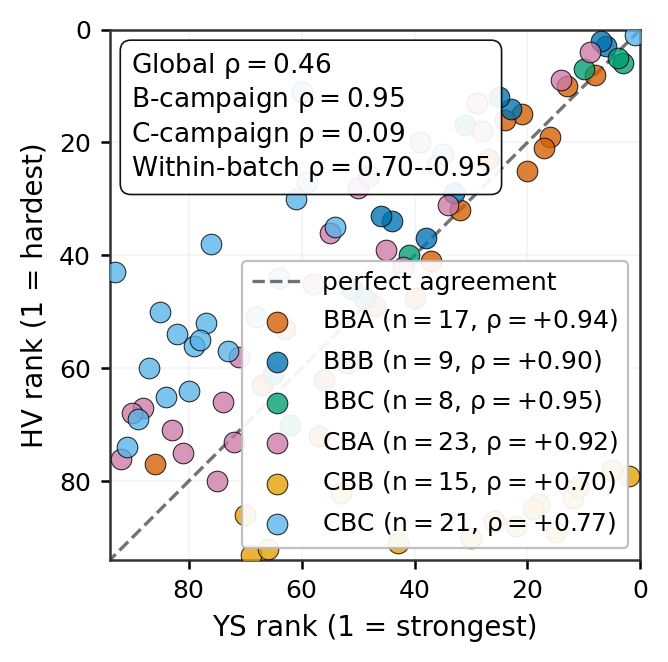
\includegraphics[width=0.68\textwidth]{fig_hv_ys_rank.png}
  \caption{HV rank versus YS rank by batch. Strong ordering within each batch becomes weaker after pooling because composition and processing coverage differ among batches.}
  \label{fig:hvrank}
\end{figure}

\section{Reproducibility across model families}
\label{si:diagnostics}

The scripts \path{verified_analysis.py}, \path{main2_validation.py}, and \path{verify_sdgrain_models.py} in \path{paper_gpt/} generate the revision-specific audit files. The second script writes \path{verified_results/main2_grouped_validation.csv}, which contains the three internal protocols used in the main paper: 5-fold, LOO, and LOBO. The third writes \path{verified_results/sdgrain_m15_validation.csv}, which independently refits M3, the additive SD control, and M15. Other verified files contain the fold-contained Family~2 PCA predictions, corrected Family~5 hardness coefficients and bootstrap intervals, the cross-batch composition audit, the E1--E3 external evidence classes, the singularity audit, and a method-claim audit.

Family~3 M15 OLS coefficients, information criteria, and grouped-CV scores are reproducible from the prepared dataset. Its earlier Bayesian stacking weight and PSIS-LOO comparison remain archival because that probabilistic analysis was not regenerated. The Family~4 nested ARMOTE-CV table remains archival because the raw folds and optimization objects are absent. Family~5 PySR remains exploratory until equation discovery is repeated within every outer training split. Full-data loadings, feature rankings, and symbolic search fronts are descriptive and should not be substituted for held-out performance.

\bibliographystyle{elsarticle-num}
\bibliography{references}
\end{document}
